\documentclass{article}

\usepackage[english]{babel}
\usepackage[utf8]{inputenc}
\usepackage{amsmath}
\usepackage{graphicx}
\usepackage[colorinlistoftodos]{todonotes}
\usepackage{amsfonts}
\usepackage{titling}
\usepackage{indentfirst}
\usepackage{adjustbox}
\usepackage{graphicx}
\usepackage{float}
\usepackage{pgfplots}

\usepackage[utf8]{inputenc}
\usepackage[english]{babel}
 
\usepackage{amsthm}
 
\theoremstyle{definition}
\newtheorem{definition}{Definition}[section]
 
\theoremstyle{remark}
\newtheorem*{remark}{Remark}
\newtheorem{theorem}{Theorem}
\newtheorem{corollary}{Corollary}

\usepackage{hyperref}
\newcommand\fnurl[2]{%
\href{#2}{#1}%
}

\graphicspath{ {images/} }
\renewcommand\maketitlehooka{\null\mbox{}\vfill}
\renewcommand\maketitlehookd{\vfill\null}

\title{An Analysis of Growth and Connection in Chicago’s Neighborhoods using Eigenvector Centrality}

\author{Benjamin Rothschild}

\date{\today}
\begin{document}
\begin{titlepage}
\maketitle
\thispagestyle{empty}

\end{titlepage}

\section{Introduction}
 
There have been many approaches to analyze job and neighborhood growth in cities that spans academic disciplines from economics to statistics and sociology.  Much research has focused on important questions like what creates jobs growth, increases home values, or decreases crime and there are many standard statistical tools researchers have in their tool belt to analyze these questions such as regression, causal frameworks, and policy evaluation.  One aspect of cities that is less studied, however, is the connection between employment centers and housing and how this network creates and distributes wealth within a city.  Approaches to quantify important links in networks have been studied in other academic areas such as trade routes, migration patterns, and social networks.  In this paper I will use a common tool used to quantify important nodes in a network, eigenvector centrality, to find important neighborhoods for employment and housing in the commuting network of Chicago.  The eigenvector centrality method of computing node importance in a network will help us understand how the relationship between employment and housing centers in Chicago and allow us to ask additional research questions such as how wealth and employment is distributed across the city and how connections between neighborhoods influence the growth of the city.  In this paper I will use the Longitudinal Employer-Household Dynamics dataset published by the US Census in order to apply this method.

\section{Literature Review}

The first researcher to apply the mathematics of eigenvectors to geography was P.R. Gould.  In his paper On the Geographical Interpretation of Eigenvalues his goal was less motivated by a specific hypothesis but more of a curiosity to determine if this mathematical structure could uncover a pattern and order in very complex situations.\footnote{add citation}  His hope, which many computational social scientists share, was that underlying complex phenomena might be a mathematical idea that could provide a meaningful geographic interpretation.  To explore this idea, he maps out the road network of Uganda and creates a connectivity matrix of this network on a binary scale, 1 indicating if two cities are connected and 0 if they are not.  He calculated the first four eigenvectors of these matrices in 1921 and 1935 and compared the results.  He found the first eigenvalue, which is centered around the city of Kampala, was by far the most connected town owning to the number of direct linkages and its central location.  The city with the next highest value, Entebbe, was also very connected.  He then examines a new connectivity matrix of the cities in 1935 and describes how several structural characteristics have been strengthened as new cities are added to the network and also notes that the successive eigenvectors and eigenvalues are a “pull out” of small regional networks within the trading structure.  Gould makes an attempt, though vague, to describe the meaning of this calculation.  He says “vectors representing well-connected towns will not only lie in the middle of a large number of dimensions but will tend, in turn, to lie close to the principal eigenvalue.  Towns that are moderately well connected will not lie in the middle of so many dimensions as the well-connected towns and will tend to form small structural clusters on their own” .  This interpretation has been named the “Gould Index of Accessibility”.\\

Other researchers have since offered definitions of eigenvalues of the connectivity matrix in geographic and social networks.  Tinkler described these eigenvalues in the context of a social network.  If there is a social network of with a rumor teller at some vertex $i$ at time 0, as time progresses, the rumor will be spread throughout the network according to the connections between people in the social network.  The distribution of the rumor by time $t$ is the equilibrium distribution after a large number of time periods will also be given by Gould’s index.   In other words, after time progresses the eigenvector is the chance that the rumor has spread to a specific node in the network. \\

Another interpretation of eigenvector centrality was given by J.W. Moon who described the eigenvalues in terms of an iterative round-robin competition between teams.  In his example, a player gets a ranking by beating another player, however if they beat a stronger player they will get a higher rating boost than if they beat a weaker player.  After the tournament has elapsed after a certain amount of turns the ranking of the player will be the same as Gould’s index.\footnote{add citation}\\

Another interesting application of eigenvector centrality was developed by Sergey Brin and Lawrence Page in creating a web search engine which served as the basis of the first version of Google’s search engine.  They created a database of the hyperlink network of over 24 million pages and a PageRank algorithm to order results of a query.  Pages are arranged in a network based on their hyperlinks to other pages.  PageRank does not count all links equally though, but normalized the weighting by the number of links on the page.  The PageRank of a webpage was calculated using an iterative algorithm that corresponded to the principal eigenvector of the normalized link matrix of the web.  They give a few intuitive justifications why this ranking works.  One was imagining a “random surfer” who is given a web page at random and keeps clicking links.  The PageRank of a page is the probability the random surfer will land on a page.  Another interpretation was that a page will have a high PageRank if there are many pages that point to it, or if there are some pages that point to it and also have a high PageRank so it was a way to combine a ranking that measured reputation and ubiquity.\\

Another important and related area of research is studying the secondary eigenvector in the network.  For example, in Gould’s analysis the second eigenvector was able to pick out significant geographic subsystems.  Often there remains further information about the network structure that subsequent eigenvectors can explain. For example, where the first eigenvector is likely to reflect volumes and strengths of connections among the actors, a second or third eigenvector can delineate those in separate groups within the network who behave in somewhat equivalent manners, or other elements of network structure that can be informative in understanding the actors and the patterns that link them. Iaocobucci et al demonstrate that the extraction of only the first eigenvector can be, and in even modest-sized networks insufficient for a more comprehensive understanding of the network.\footnote{cite this}  The example they give is from a communication network between researchers.  While the first eigenvector retrieves the principal structure of the social network it is often similar to common measures of centrality.  By extracting the second and third eigenvector several classes of network structures and actor attributes were clearly pulled out and interpreted.  This is because if the first eigenvector the second eigenvector by necessity will be uncorrelated with the previous eigenvectors and therefore uncorrelated with the traditional degree of centrality.  This lack of redundancy indicates the supplemental information that the eigenvector can bring to the network modeler.  In my analysis I will also try to explain the interpretation of the first and second eigenvectors.

\section{Data}
The main dataset I am using in my analysis is the Longitudinal Employer-Household Dynamics Dataset (LEHD) that is published by the United States Census Bureau.  This is a synthetic dataset that joins firm employment data and census demographic data on the census block level and provides a fine-grained view of the connections between where people live and work.  This is an innovative way for a government to release data and has many benefits as it creates an interesting dataset at a low cost since it leverages existing datasets and there is no additional burden on respondents such filling out additional surveys.  The datasets that are used to produce the LEHD dataset include, Unemployment Insurance wage records, the Quarterly Census of Employment and Wages, and the Statistical Administrative Records System.  Some of the data sources that are used to produce the LEHD dataset are confidential and not themselves made public.  The current coverage of employment data is limited to jobs covered by the Unemployment Insurance Program which is approximately 95\% of jobs in the United States.  \\

Jobs are broken down among job categories, employee age brackets, and employee monthly salary as follows:
\begin{enumerate}
\item Job Category:
    \begin{enumerate}
        \item Goods Producing
        \item Trade, Transportation, and Utilities
        \item Other
    \end{enumerate}
\item Age:
    \begin{enumerate}
        \item 29 and younger
        \item 30 - 45
        \item 55 and older
    \end{enumerate}
\item Monthly Salary:
    \begin{enumerate}
        \item under \$1,250
        \item \$1,251 - \$3,333
        \item over \$3,333
    \end{enumerate}
\end{enumerate}

The data is published every year from 2002 to 2015.\footnote{Data is available for almost all State-Year combinations except around 9 which the Census department notes there are data integrity issues.  Illinois was not noted on this list, so my study is unaffected by missing data.}  The data that is published shows the number of people who live and work between each census block in the United States.  Census blocks are currently the smallest geographic units used in the US Census Bureau statistics.  The number of census blocks in the 2010 Census was 11,155,486 with an average size of 1,500 people so the resultant dataset provides a very fine-grained view of the relationship between places of work and employment.  Since the data is so fine-grained the Census Bureau employs a few techniques to protect confidentiality of the users such as noise infusion and other synthetic methods using probabilistic differential privacy. \footnote{More information about noise infusion and confidentially protection can be found on the \fnurl{census website}{https://www2.census.gov/ces/wp/2014/CES-WP-14-30.pdf}}.\\

In my analysis I focus on data within the Chicago Metropolitan Statistical Area and a summary of the employment data for the 2002 is below. \\
\begin{center}
 \begin{tabular}{|| c | c | c||} 
 \hline
 & Count & Percent of Total \\[0.5ex] 
 \hline\hline
 Total Jobs & 3,924,152  & 100\% \\  \hline
 Age: 29 or younger & 1,027,445 & 26.1\% \\ 
 Age: 30 to 54 & 2,328,093 & 59.3\% \\
 Age: 55 or older & 568,614 & 14.4\% \\ \hline
 Earnings: \$1250month or less & 1,090,632 & 27.7\% \\ 
 Earnings: \$1251/month to \$3333/month  & 1,467,733 & 37.3\% \\ 
 Earnings: greater than \$3333/month & 1,365,787 & 34.7\% \\ \hline
 Goods Producing  & 708,324 & 18.0\% \\ 
 Trade, Transportation, and Utilities  & 819,502 & 20.8\% \\ 
 Other  & 2,396,326 & 61.6\% \\ \hline 
\end{tabular}
\end{center}

The basis of my analysis is based off of the eigenvector centrality of the live-work commuting matrix between census tracts in Chicago.  Though the LEHD dataset provides census tract level statistics I found that interpretability improves at a slightly larger area so decided to use census blocks and neighborhoods of which there are 2,215 and 190 respectively in the Chicago metropolitan statistical area. To visualize the dataset, I first created a connectivity graph between all census tracts with more than 25 people commuting between them shown below.\\


\begin{figure}[H]
    \centering
    \includegraphics[width=1.0\textwidth]{arc-1}
    \caption{This map shows all the connections between where people live and work in Chicago.}
    \label{fig:arc-1}
\end{figure}

\begin{figure}[H]
    \centering
    \includegraphics[width=1.0\textwidth]{arc-2}
    \caption{This map shows the connections between a people living Hyde Park who either commute to the University of Chicago or the The Loop}
    \label{fig:arc-2}
\end{figure} \\

I use data from Zillow to measure housing values.  Zillow produces data at the neighborhood level for a number of statistics.  The datasets I look at are produced monthly from .  I look at two measures \% of houses increasing in value and median home value per square foot.\\

I use the building permits and building licenses dataset published by the City of Chicago Department of Buildings in order to measure investments in business properties in the city.  This dataset is available from 2006 to the present.  Along with each permit application are the following fields Permit type, Date, Estimated Cost, Street Address, Work Description.  A visualization of the dataset for data in 2005 is below. TODO


\section{Methods}
In order to find the employment centers of a city I will use a setup based on eigenvector centrality that has been used in studying networks such as trade routes, social networks, and webpages.  The goal of the method is to take a network of linked entities and to output the most influential nodes in the network graph.  The definition of influential varies depending on the context of how the problem is set up and what the nodes and edges represent.  For example, in a social network, the most important node is the person who is connected to the most important people or in the “center”.  In a network of cities that trade with each other, the edges might represent the distance between cities.  The edges can either represent a connection, in which case the matrix is called an adjacency matrix and is filled with 1 and 0’s depending on if two nodes are connected to each other or the matrix could represent the strength of connection between two nodes, for example in the trading routes example it could be the distance between two cities.  In this case it is common to normalize the distances to the sum of each column is equal to one. \\

Before I demonstrate how the network matrix is built in the context of this paper, it is important to understand why we are guaranteed a positive eigenvalue from the following theorem proven by Oskar Perron and Georg Forbenius.

\theoremstyle{definition}
\begin{theorem}[Perron-Frobenius Theorem]
\label{Perron-Frobenius Theorem}
Let $C$ $\in$ $\mathbb{R}^{nxn}$ represent a nonnegative primitive matrix (i.e. $C$: $C_{i,j}$ $>$ 0).  There exists a positive real number $\lambda_{max}$, such that:
\begin{enumerate}
\item $\lambda_{max}$ $>$ 0
\item $\lambda_{max}$ has a unique (up to a constant) eigenvector $v$ which has all positive entries
\item $\lambda_{max}$ $>$ $|\lambda|$ for any eigvenvalue $\lambda$ $\neq$ $\lambda_{max}$
\end{enumerate}

\end{theorem}
TODO: proof?

\begin{theorem}
A column stochastic matrix will always has an eigenvalue 1. All other eigenvalues are in absolute
value smaller or equal to 1.
\end{theorem}
TODO: proof?
\\ 

To illustrate the network I will explore in my paper, consider a simplified example of a city of 110 people, 100 of whom live Downtown and 10 of whom live in Hyde Park.  Of the 100 people who live downtown, 90 works downtown and 10 works in Hyde Park while of the 10 people, 5 work downtown and 5 work in Hyde Park.  This network can be represented by the following matrices. 

\begin{equation}
      C
   =
  \begin{bmatrix}
    hyde park->hyde park  & hyde park->downtown\\
    downtown->hyde park  & downtown->downtown
    
  \end{bmatrix} = 
  \begin{bmatrix}
    5 & 10\\
    5 & 90 
  \end{bmatrix}
\end{equation}

\begin{equation}
      l
   =
  \begin{bmatrix}
    hyde park\\
    downtown
    
  \end{bmatrix} = 
  \begin{bmatrix}
    10\\
    100 
  \end{bmatrix}
\end{equation}

\begin{equation}
      w
   =
  \begin{bmatrix}
    hyde park\\
    downtown
  \end{bmatrix} = 
  \begin{bmatrix}
    15\\
    95
  \end{bmatrix}
\end{equation}

From this information we can create a commuting matrix which normalizes the flow between regions of the city and transforms the “live” matrix (2) into the “work” matrix (3).  This transforms the above matrices into the following equation.

\begin{equation}C w = l\end{equation}
\begin{equation} 
  \begin{bmatrix}
    5/15 & 5/95\\
    10/15 & 90/95
  \end{bmatrix}
  \begin{bmatrix}
    15\\
    95
  \end{bmatrix}
  = 
  \begin{bmatrix}
    10\\
    100
  \end{bmatrix}
\end{equation}

We can also calculate write out the commuting flow from work to home as

\begin{center}C $l$ = $w$\end{center}
\begin{equation} 
  \begin{bmatrix}
    0.5 & 0.1\\
    0.5 & 0.9
  \end{bmatrix}
  \begin{bmatrix}
    10\\
    100
  \end{bmatrix}
  = 
  \begin{bmatrix}
    15\\
    95
  \end{bmatrix}
\end{equation}

Lastly, I will create a network from the dataset which represents a theoretical economy within the city.  Instead of people, I consider the flow of money between regions modeled by the salary of workers that commute between regions.  The first model will be the total flow of money between regions represented by the sum of the salaries of all the workers who commute between regions.  For example, if 10 people commute from Hyde Park to Downtown and they each make an average of \$2,500 per month I will consider the money flow between Hyde Park and downtown to be \$25,000.  In my dataset, salaries are broken down into three ranges less than \$1,250, \$1,250-\$3,333 and over \$3,333.  To simplify the problem, I will represent the buckets as \$1,250, \$2,500, and \$5,000.  Consider the same commuting flows as above but now with income added according to the following breakout.\\

\begin{adjustbox}{center}
 \begin{tabular}{||c | c c c | c | c | c||} 
 \hline
 & \$1,250 & \$2,500 & \$5,000 & Total People & Total Salaries\\[0.5ex] 
 \hline\hline
 $Hyde Park -> Hyde Park$ & 1 & 2 & 2 & 5 & \$16,250 \\ 
 $Hyde Park -> Downtown$ & 2 & 3 & 5 & 10 & \$35,000 \\
 $Downtown -> Hyde Park$ & 0 & 1 & 4 & 5 & \$22,500 \\ 
 $Downtown -> Downtown$ & 10 & 20 & 60 & 90 & \$362,500 \\ 
 \hline
 \end{tabular}
\end{adjustbox}\\ \\

This is represented by the following matrix.\\

\begin{equation}
  C =
  \begin{bmatrix}
   Salaries_{HP->HP}  & Salaries_{HP->D}\\
   Salaries_{D->HP}  & Salaries_{D->D}
    
  \end{bmatrix} = 
  \begin{bmatrix}
    \$16,250 & \$35,000\\
    \$22,500 & \$362,500 
  \end{bmatrix} = 
  \begin{bmatrix}
    .419 & .088\\
    .580 & .912
  \end{bmatrix}
\end{equation}
\\
Next, I take the $C$ matrix in (5), (6), \& (7) and computing the corresponding eigenvectors and eigenvalues.\\

\begin{center}
Eigenvalue and Eigenvector for (5) \\
\begin{tabular}{||c | c c ||} 
 \hline
 & $\lambda_1$ = 1.0 & $\lambda_2$ = 0.28\\[0.5ex] 
 \hline\hline
 $Downtown$ & 0.99689815 & 0.07870249 \\
 $Hyde Park$ & 0.70710678 & -0.70710678  \\ 
 \hline
 \end{tabular} \\ 
Eigenvalue and Eigenvector for (6) \\
\begin{tabular}{||c | c c ||} 
 \hline
 & $\lambda_1$ = 1.0 & $\lambda_2$ = 0.4\\[0.5ex] 
 \hline\hline
 $Downtown$ & 0.98058068 & 0.19611614 \\
 $Hyde Park$ & 0.70710678 & -0.70710678  \\ 
 \hline
 \end{tabular} \\ 
Eigenvalue and Eigenvector for (7) \\
\begin{tabular}{||c | c c ||} 
 \hline
 & $\lambda_1$ = 1.0 & $\lambda_2$ = 0.33\\[0.5ex] 
 \hline\hline
 $Downtown$ & 0.98869689 & 0.14992818 \\
 $Hyde Park$ & 0.70710678 & -0.70710678  \\ 
 \hline
 \end{tabular}
 \end{center}

These results will demonstrate a few things.  First note that the principle eigenvalue is 1.0 as expected from the theorem above.  The vector that corresponds to the principle eigenvalue is the Gould Index of Accessibility in the network and represents the relative strength of each node in the principle network.  In the three examples above you can see that the Downtown area dominates this vector.  The second eigenvalue represents a "pull out" of the principle network.  It is important to remember that the second eigenvector will be orthogonal to the principle eigenvector and represents a completely different sub-network.  In the system in equation 5 and 7 the second eigenvalue is lower which indicates the dominance of the first eigenvalue compared to the network examined in the 6 equation.  These results have a similar interpretation to the previous example where the principle eigenvector show the most dominant network of living regions.  The eigenvector that corresponds to the principle eigenvalue are the relative ranking of regions in this setting.  Next I will use this same set up to analyze the neighborhoods of Chicago using the LEHD dataset.

\section{Results}
\subsection{Centrality for Employment}
First, I will study what neighborhoods are the most important for different job sectors, income ranges, and age profiles.  I will use the commuting matrix described in equation 6 to rank the neighborhoods according to the eigenvector that corresponds to the principle eigenvalue.  Answering the question \textit{How important is a neighborhood to jobs in a specific industry, age group or salary range?}  To do this, I create a connectivity matrix over all neighborhoods in the Chicago MSA and rank them from the years 2002 - 2015.  Below I list the top 10 neighborhoods ranked according to the eigenvalue that corresponds to the principle eigenvector.  In the last column I note the percentage change from 2002 to 2015 of the neighborhood. \\

\begin{adjustbox}{center}
\begin{tabular}{||c | c c c c c c c c c c c c c c | c||} 
 \hline
 & 2002 & 2003 & 2004 & 2005 & 2006 & 2007 & 2008 & 2009 & 2010 & 2011 & 2012 & 2013 & 2014 & 2015 & \%\\[0.5ex] 
 \hline\hline
The Loop       & 0.958 & 0.952 & 0.954 & 0.939 & 0.947 & 0.955 & 0.947 & 0.960 & 0.961 & 0.962 & 0.962 & 0.964 & 0.962 & 0.964 & +0.60\% \\
Streeterville  & 0.162 & 0.176 & 0.180 & 0.203 & 0.206 & 0.168 & 0.174 & 0.157 & 0.146 & 0.144 & 0.134 & 0.131 & 0.115 & 0.129 & -20.4\% \\
O'Hare Airport & 0.121 & 0.084 & 0.079 & 0.078 & 0.057 & 0.079 & 0.120 & 0.063 & 0.077 & 0.070 & 0.090 & 0.074 & 0.095 & 0.082 & -32.3\% \\
South Loop     & 0.102 & 0.124 & 0.113 & 0.125 & 0.115 & 0.110 & 0.114 & 0.109 & 0.075 & 0.081 & 0.086 & 0.089 & 0.090 & 0.065 & -37.0\% \\
River North    & 0.074 & 0.070 & 0.076 & 0.084 & 0.083 & 0.082 & 0.085 & 0.079 & 0.097 & 0.091 & 0.098 & 0.094 & 0.099 & 0.116 & +56.8\% \\
Bronzeville    & 0.041 & 0.036 & 0.049 & 0.056 & 0.016 & 0.044 & 0.050 & 0.048 & 0.037 & 0.034 & 0.011 & 0.014 & 0.013 & 0.011 & -73.2\% \\
Near North     & 0.074 & 0.098 & 0.085 & 0.101 & 0.098 & 0.091 & 0.088 & 0.088 & 0.085 & 0.086 & 0.073 & 0.070 & 0.073 & 0.074 & +0.00\% \\
West Loop Gate & 0.073 & 0.084 & 0.083 & 0.097 & 0.085 & 0.087 & 0.087 & 0.085 & 0.083 & 0.094 & 0.089 & 0.094 & 0.099 & 0.105 & +43.8\% \\
West Town      & 0.039 & 0.052 & 0.049 & 0.052 & 0.054 & 0.048 & 0.049 & 0.049 & 0.041 & 0.045 & 0.046 & 0.042 & 0.047 & 0.053 & +35.9\% \\
Archer Heights & 0.034 & 0.039 & 0.032 & 0.033 & 0.034 & 0.027 & 0.031 & 0.025 & 0.028 & 0.019 & 0.014 & 0.013 & 0.022 & 0.019 & -44.2\% \\
Hyde Park      & 0.049 & 0.043 & 0.063 & 0.092 & 0.077 & 0.080 & 0.100 & 0.067 & 0.096 & 0.087 & 0.094 & 0.088 & 0.088 & 0.089 & +81.6\% \\
 \hline
 \end{tabular}
\end{adjustbox}
\\

\begin{figure}[H]
    \centering
    \includegraphics[width=0.31\textwidth]{Jobs-S000-2002}
    \includegraphics[width=0.31\textwidth]{Jobs-S000-2008}
    \includegraphics[width=0.31\textwidth]{Jobs-S000-2015}

        
    \caption{This map shows the eigenvector corresponding to the principle eigenvalue for 2002, 2008, and 2015}
    \label{fig:Jobs-S000-2008}
\end{figure}

As can be seen in the map and table employment is Chicago is highly concentrated in the downtown The Loop neighborhood which consistently is ranked above .95 and dominating the rank of all other neighborhoods.  Other consistently important neighborhoods include include Streeterville which is just north of The Loop as well as O'Hare Airport. Looking at the change in rankings overtime can give us an interesting view of how neighborhoods are becoming more or less important centers of employment over time.  For example, West Loop gate which is the neighborhood just west of the Chicago River has become much more important relative to other neighborhoods.  There have been a number of high tech companies that have opened offices in the West Loop since 2014 such Uber and Google to name a few.\footnote{https://www.builtinchicago.org/2014/09/18/meet-neighbors-4-tech-companies-sign-huge-leases-west-loop}.  Hyde Park has also grown in importance driven by the census blocks that cover the University and Harper Court.\footnote{https://fiftythird.uchicago.edu/category/tags/harper-court-partners} \footnote{this feels anecdotal, bring in the other LEHD employment data, how is this conclusion different from just analyzing the counts?}\\

Another interesting view of the data is to look at the value and location of the second eigenvector of the network over time.  As explained before the second eigenvector will depict a completely orthogonal network compared to the primary eigenvector and can give an idea of how more or less important the primary network is than the next network. One way to think of the second eigenvector would be a completely different "economy" that is somehow separate from the primary "economy" in the city, for example it is common for people to live between these regions with less access to the primary region.  In the graph below I show the value of the second eigenvalue over time which decreases from 0.51 to 0.41 from 2002 to 2015.  This means that compared to the primary network the influence of the secondary network is decreasing.  There could be a few reasons for this, for example the primary network could be increasing in size from outside forces or perhaps people from the secondary network are joining the primary network.  An alternative explanation is that people are leaving the secondary network. TODO: any way to show this?\\
\begin{center}
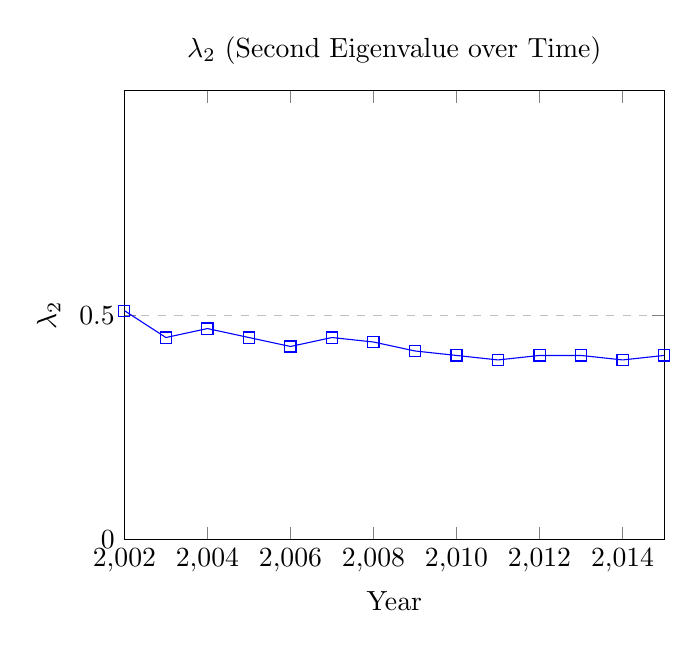
\begin{tikzpicture}
\begin{axis}[
    title={$\lambda_2$ (Second Eigenvalue over Time)},
    xlabel={Year},
    ylabel={$\lambda_2$},
    xmin=2002, xmax=2015,
    ymin=0, ymax=1,
    xtick={2002, 2004, 2006, 2008, 2010, 2012, 2014},
    ytick={0, 0.5},
    legend pos=north west,
    ymajorgrids=true,
    grid style=dashed,
]
 
\addplot[
    color=blue,
    mark=square,
    ]
    coordinates {
    (2002, 0.51)
    (2003, 0.45)
    (2004, 0.47)
    (2005, 0.45)
    (2006, 0.43)
    (2007, 0.45)
    (2008, 0.44)
    (2009, 0.42)
    (2010, 0.41)
    (2011, 0.40)
    (2012, 0.41)
    (2013, 0.41)
    (2014, 0.40)
    (2015, 0.41)
    };

\end{axis}
\end{tikzpicture}
\end{center}

Next I will take a look at how the different neighborhoods specialize in different jobs.  Below I map the primary eigenvalue for all job categories, ages, and income levels in three years, 2002, 2008, and 2015.

\begin{figure}[H]
    \centering
    \includegraphics[width=0.31\textwidth]{Jobs-SI001-2015}
    \includegraphics[width=0.31\textwidth]{Jobs-SI002-2015}
    \includegraphics[width=0.31\textwidth]{Jobs-SI003-2015}
    \caption{These maps show the eigenvectors for the three different industry categories: Goods Producing (left), Trade, Transportation, Utilities (center), Other (right) for 2015}
    \label{fig:Jobs-S000-2008}
\end{figure}

This method of centrality importance is clearly able to pull out the different networks of employment in Chicago such as how dispersed the Goods Producing sector is compared to the Trade, Transportation, and Utilities sector which is dominated by O'Hare International Airport.  The Other category is dominated by The Loop area where most of the jobs in the city are located. \\

Lastly I will look at the centrality importance of jobs at different income levels.

\begin{figure}[H]
    \centering
    \includegraphics[width=0.31\textwidth]{Jobs-SE001-2015}
    \includegraphics[width=0.31\textwidth]{Jobs-SE002-2015}
    \includegraphics[width=0.31\textwidth]{Jobs-SE003-2015}
    \caption{These maps show the eigenvectors for the three different salary levels: Under \$1,250 left, \$1,250 - \$3,333 center, Over \$3,333 right for 2015.}
    \label{fig:Jobs-S000-2008}
\end{figure}

Note:  It is interesting that these three maps look very similar however I'm not sure that this is the best way to analyze the data.  It might be better to compare the values for the eigenvector in a neighborhood between the three income bracket?  For example, is a neighborhood more prominent for high income jobs vs low income jobs?  Look into this more...

Above I used the theory of eigenvector centrality to rank the most important neighborhoods of employment for neighborhoods in Chicago.  This perspective gives us a rich view of the composition of a neighborhood as well as how it changes over time in comparision to other neighborhoods in the city.

\subsection{Centrality for Housing}
Similar to how we calculated centrality for employment we can use the same setup to calculate the centrality for housing, answering the question \textit{What neighborhoods are the most important for housing?}.  We can also break down the neighborhoods by most important for High/Middle/and Low income earners based off of the LEHD Dataset.  The top neighborhoods 10 neighborhoods based on their centrality from 2002 are listed below. \\

\begin{adjustbox}{center}
\begin{tabular}{||c | c c c c c c c c c c c c c | c ||} 
 \hline
 & 2002 & 2003 & 2005 & 2006 & 2007 & 2008 & 2009 & 2010 & 2011 & 2012 & 2013 & 2014 & 2015 & | \%\\[0.5ex] 
 \hline\hline
Logan Square      & 0.303 & 0.307 & 0.296 & 0.287 & 0.207 & 0.296 & 0.201 & 0.313 & 0.316 & 0.323 & 0.333 & 0.340 & 0.322 & +6.27\% \\
Englewood         & 0.247 & 0.244 & 0.236 & 0.239 & 0.258 & 0.223 & 0.252 & 0.197 & 0.185 & 0.178 & 0.172 & 0.177 & 0.179 & -27.6\% \\
Gresham           & 0.238 & 0.239 & 0.233 & 0.231 & 0.245 & 0.242 & 0.254 & 0.202 & 0.205 & 0.213 & 0.193 & 0.201 & 0.215 & -10.7\% \\
West Rogers Park  & 0.220 & 0.221 & 0.224 & 0.230 & 0.201 & 0.221 & 0.209 & 0.246 & 0.260 & 0.261 & 0.254 & 0.245 & 0.239 & +8.63\% \\
Little Village    & 0.208 & 0.200 & 0.196 & 0.193 & 0.201 & 0.176 & 0.201 & 0.178 & 0.171 & 0.183 & 0.187 & 0.197 & 0.188 & -9.70\% \\
Albany Park       & 0.189 & 0.195 & 0.179 & 0.172 & 0.144 & 0.181 & 0.133 & 0.186 & 0.198 & 0.201 & 0.193 & 0.183 & 0.179 & -5.30\% \\
Portage Park      & 0.188 & 0.185 & 0.181 & 0.182 & 0.214 & 0.191 & 0.220 & 0.201 & 0.203 & 0.190 & 0.198 & 0.188 & 0.189 & +0.50\% \\
Archer Heights    & 0.181 & 0.178 & 0.186 & 0.182 & 0.187 & 0.173 & 0.185 & 0.198 & 0.173 & 0.175 & 0.184 & 0.186 & 0.188 & +3.86\% \\
Brighton Park     & 0.165 & 0.170 & 0.167 & 0.166 & 0.141 & 0.157 & 0.135 & 0.151 & 0.149 & 0.148 & 0.159 & 0.165 & 0.162 & -1.90\% \\
Back of the Yards & 0.159 & 0.153 & 0.165 & 0.166 & 0.152 & 0.156 & 0.150 & 0.159 & 0.140 & 0.144 & 0.149 & 0.149 & 0.148 & +7.00\% \\
 \hline
 \end{tabular}
\end{adjustbox}
\\

Some things to notice right away are that the rankings are much more stable than they were for the employment dataset, most neighborhoods only increasing or decreasing in the single digits over the 14 year timespan.  Also, the distributions of the rankings are a lot more even across neighborhoods compared to the employment dataset which was dominated by The Loop neighborhood. 

\begin{figure}[H]
    \centering
    \includegraphics[width=1.0\textwidth]{Houses-S000-2015}
    \caption{This map shows the eigenvector that corresponds to the principal eigenvalue for the housing pagerank algorithm.}
    \label{fig:Houses-S000-2015}
\end{figure}

\subsection{Centrality for Money Flow}
I am currently working on the computation for this section.  The idea is outlined in the methods section where I will calculate neighborhood importance based off of the money that flow between neighborhoods (this is based on salary * number of workers).  I will also add outside data from construction permits etc to help with this analysis.
\section{Conclusion}
\section{Citations}
\section{To Do}
\begin{enumerate}
\item Section 5.3 (+3 pages)
\item Abstract (+.5 page)
\item Conclusion (+.5 page)
\item Citations in LaTeX (+1 page)
\item Clean out unreferenced/other data on website
\item add final jupyter notebooks to github
\item more on computation \& data processing process? (+.5 page)
\item describe zillow data (+.75 page)
\item describe building data (+.75 page)
\end{enumerate}

\end{document}








